\documentclass[12pt, a4paper]{article}


\usepackage[german]{babel}
\usepackage[ansinew]{inputenc}
\usepackage[T1]{fontenc} %Umlaute
\usepackage{lmodern}
\usepackage[top=2cm, left=4cm, bottom=2cm, right=3cm]{geometry}
\usepackage{graphicx}
\usepackage{listings} 
\usepackage{multirow}
\usepackage{color}		 % f�r Farben im allgemeinen
\usepackage{colortbl}
\usepackage{cite}
\usepackage{bibgerm}
\usepackage{palatino}
\usepackage{chngpage}
\renewcommand{\floatpagefraction}{0.85}

\usepackage{fancyhdr}
\pagestyle{fancy}



\fancyhf{}
\fancyhead[RE]{\slshape \nouppercase{\leftmark}}    % Even page header: "page   chapter"
\fancyhead[LO]{\slshape \nouppercase{\rightmark}}   % Odd  page header: "section   page"
\fancyhead[RO,LE]{\bfseries \thepage} 
\renewcommand{\headrulewidth}{1pt}    % Underline headers
\renewcommand{\footrulewidth}{0pt}    

\fancypagestyle{plain}{               % No chapter+section on chapter start pages
\fancyhf{}
\fancyhead[RO,LE]{\bfseries \thepage}
\renewcommand{\headrulewidth}{1pt}
\renewcommand{\footrulewidth}{0pt}
}

% Left headings: "1  INTRODUCTION"
%\renewcommand{\chaptermark}[1]{%
%\markboth{\thechapter\ \ \ \ #1}{}}

% Right headings: "1.1  Basics"
\renewcommand{\sectionmark}[1]{%
\markright{\thesection\ \ \ \ #1}{}}

\lstset{language=java} 
\lstset{basicstyle=\scriptsize}
\lstset{numbers=left, numberstyle=\tiny, numbersep=2pt, breaklines=true} 
\graphicspath{{Bilder/}}
\newcommand{\listoflolentryname}{\lstlistingname} 
%\newcommand{\fullcite}{\citep} %for "Author [1980]"
\usepackage[pdftex,plainpages=false,pdfpagelabels]{hyperref}
% --- Farbdefinitionen ----------------------------------------
\definecolor{rot}{rgb}{1,0.3,0}
\definecolor{gelb}{rgb}{1,1,0}
\definecolor{gruen}{rgb}{0,1,0.4}
\definecolor{darkblue}{rgb}{0.2,0.3,1}
\definecolor{lightblue}{rgb}{0.6,0.7,1}
\definecolor{white}{rgb}{1,1,1}

\linespread{1.5}

\bibliographystyle{geralpha}

%----------------------------------------------------------------------------------
% \vcite	
%				{ source }
%				{ page }
%
%Direktes Zitat
\newcommand{\simplevcite}[1]
{
(vgl. \cite{#1})
}

%----------------------------------------------------------------------------------
% \vcite	
%				{ source }
%				{ page }
%
%Direktes Zitat
\newcommand{\vcite}[2]
{
(vgl. \cite[S.#2]{#1})
}


\begin{document}

%\frontmatter

%\frontmatter

%Die Titelseite aus dem "images"-Verzeichnis wird verwendet
\begin{titlepage}
%Das Originaltemplate nutzt
%\AddToShipoutPicture*{
%\put(0,0){
%\includegraphics[width=\paperwidth]{titlepage}}}
%\strut

\includegraphics[width=\textwidth]{nak.png}
\begin{center}
\parskip5mm
\large P R A X I S B E R I C H T
%\normalsize in der Fachrichtung\\
% Wirtschaftsinformatik
 
\large T H E M A

\parbox{11cm}{
\begin{center}
\LARGE\textbf{Analyse von Arbeitserleichterungen durch die Nutzung von xText im Workflow zur Konfiguration von Pflichtpr�fungen f�r profil c/s }
\end{center}
}
\normalsize
\begin{tabular}{ll}
Eingereicht von: &Niels Gundermann \\% (Matrikelnr. 3418)\\
%&Woldegker Stra�e 34\\
%&17033 Neubrandenburg\\
%&Tel.: 0395/37961338\\
%&E-Mail: anna-schroeder@web.de\\
%&\\
%Erarbeitet im: &7. Semester\\
%&\\
%Abgabetermin: &18. Februar 2011\\
%&\\
%Gutachter:&Prof. Dr. Frank Zimmermann\\
%&\\
%Co-Gutachter:&Prof. Dr. Johannes Brauer\\
%&\\
%Betrieblicher Gutachter:&Dipl.-Ing. Stefan Post\\ 
%&Woldegker Stra�e 12\\
%&17033 Neubrandenburg\\
%&Tel.: 0395/5630553\\
%&E-Mail: stefan.post@data-experts.de\\
\end{tabular}
\end{center}
\end{titlepage}
\pagebreak
\pagenumbering{Roman}

\tableofcontents
\pagebreak

\addcontentsline{toc}{section}{\listfigurename}
\listoffigures
\pagebreak

\addcontentsline{toc}{section}{\listtablename}
\listoftables
\pagebreak

\lstlistoflistings
\addcontentsline{toc}{section}{Listings}
\pagebreak


%\mainmatter
\pagenumbering{arabic}
\section{Einleitung}
Gesch�ftsprozessplanung und -optimierung in einem Unternehmen haben zum Ziel,
die Kosten eines Produktes zu senken, die Produktionszeit herabzusetzen oder die Qualit�t zu
verbessern.\cite[S. 56]{gpqm} Eine Optimierung kann mit unterschiedlichen
Mitteln erreicht werden. Beispielsweise k�nnen neue und effizientere
Arbeitsverfahren eingesetzt werden. Auch die Verwendung anderer oder neuerer
Tools und Frameworks, k�nnen dem Bearbeiter Routinearbeiten abnehmen.\\
In diesem Bericht soll analysiert werden, inwiefern \emph{Xtext} f�r die data
experts gmbH (deg) in Bezug auf Kosten- und Zeiteinsparung von Nutzen ist.
\subsection{Vorgehen}
Nach Abgrenzung einiger Begriffe wird ein entsprechender Gesch�ftsprozess aus
der deg erkl�rt. Die Arbeitsabl�ufe werden dahingehend untersucht, ob \emph{Xtext} theoretisch zur Anwendung kommen kann. Anschlie�end wird analysiert wie
\emph{Xtext} konkret in den entsprechenden Arbeitsabl�ufen zu einer Kosten- oder Zeiteinsparung f�hren k�nnte.

\section{Grundlegende Begriffe}
In Kapitel \ref{GP} wird Bezug auf die Begriffe
\emph{Gesch�ftsprozess (Prozess)} und \emph{Workflow} genommen. Aus diesem Grund
wird hier eine Abgrenzung zwischen den beiden Begriffen vorgenommen. Weiterhin
werden in Kapitel \ref{Analyse der Arbeitserleichterung} die Begriffe
\emph{Syntax} und \emph{Semantik} verwendet. Wie diese Begriffe in diesem
Bericht zu verstehen sind, ist ebenfalls in diesem Kapitel definiert.

\subsection*{Gesch�ftsprozess}
Unter einem Gesch�ftsprozess (Prozess) versteht man eine Zusammenfassung der
erforderlichen betrieblichen Abl�ufe, die zur Erstellung
von Produkten und Dienstleistungen notwendig sind.\vcite{gpm}{4}
Bei der Darstellung mittels der EPK\footnote{Ereignisgesteuerte Prozesskette}
(welche in diesem Bericht verwendet wird) werden Prozesse durch Zust�nde und
Funktionen visualisiert.

\subsection*{Workflow}
Ein Workflow beschreibt die beteiligten Personen und
die von ihnen auszuf�hrenden Arbeitsschritte innerhalb des
Prozesses.\cite{workflow} Es handelt sich um eine genaue Beschreibung
der Arbeitsschritte, die abgearbeitet werden m�ssen, um den Prozess von Anfang bis
Ende durchzuf�hren.

\subsection*{Syntax}
Die Syntax ist ein Bestandteil einer Sprache. Durch die Syntax wird die Notation
der Sprache definiert. Sie beschreibt demnach die Sprachkonstrukte die f�r eine
Sprache zul�ssig sind und mit denen man sich in dieser Sprache ausdr�cken kann.
In Bezug auf Programmiersprachen beschreibt die Syntax somit die
Sprachkonstrukte, mit denen der Nutzer ein Programm beschreiben
kann.\vcite{voelter}{26} Zur Beschreibung einer Syntax wird eine
\emph{Grammatik} verwendet\footnote{Beschreibung einer Grammatik ist im
Praxisbericht \emph{Entwicklung einer
Grammatik f�r eine DSL mit xText am Beispiel einer Sprache zur Definition von 
Pflichtpr�fungen in profil c/s}\cite{pb5} zu finden.}.\vcite{theoinfo}{26}

\subsection*{Semantik}
Die Semantik ist ebenfalls ein Bestandteil einer Sprache. Sie enth�lt die Regeln
f�r die strukturelle Zusammensetzung der Sprachkonstrukte, die von der Syntax
definiert werden. Bezogen auf Programmiersprachen beschreibt die Semantik die
Bedeutung aufeinander folgender Sprachkonstrukte. \vcite{voelter}{26}

\subsection*{Xtext}
\emph{Xtext} ist ein Framework mit dem es einerseits m�glich ist, in sehr kurzer
Zeit neue Sprachen zu entwickeln. Andererseits bietet es auch f�r
bestehende Sprachen in Verbindung mit Eclipse ein entsprechendes Tooling an, mit dem sich die Arbeit
mit dieser Sprache effizienter gestalten l�sst. Das �u�ert sich darin, dass
mit \emph{Xtext} Editoren generiert werden k�nnen die Fehler in der Sprache
erkennen und den Nutzer darauf hinweisen. Diese Fehler werden dabei wie gewohnt
in der Eclipse IDE angezeigt.\vcite{xtextdoc}{113}

\section{Beschreibung des Prozesses}\label{GP}
F�r diese Analyse wurde der Prozess zur Umsetzung einer Pflichtpr�fung innerhalb
von profil c/s herangezogen.\footnote{Informationen �ber \emph{Pflichtpr�fungen}
und \emph{profil c/s} sind im Praxisbericht: \emph{Entwicklung einer Grammatik
f�r eine DSL mit xText am Beispiel einer Sprache zur  Definition von
Pflichtpr�fungen in profil c/s}\cite{pb5} zu finden.} Dieser Prozess umfasst
alle Workflows von der Anforderung des Kunden, �ber die Analyse und Implementierung der Pflichtpr�fung bis hin zur Abnahme der Umsetzung durch den Kunden. Um die �bersicht zu behalten ist es
sinnvoll den Gewsamtprozess in drei Teilprozess einzuteilen, die in den
nachfolgenden Unterkapiteln beschrieben werden.


\subsection{Anforderung und Analyse}\label{TP1}
Am Anfang des Prozesses steht immer eine Anforderung vom Kunden, die in der deg
Analysiert werden muss. Die deg erstellt f�r diese Anforderung ein
entsprechendes Angebot. In diesem Beispiel wird davon ausgegange, dass zur
Umsetzung der Anforderung eine neue Pflichtpr�fung implementiert werden muss.
Nach der Annahme des Angebotes durch den Kunden, ist dieser Teilprozess
(Abbildung \ref{Anforderung und Analyse}) beendet. 
\begin{figure}
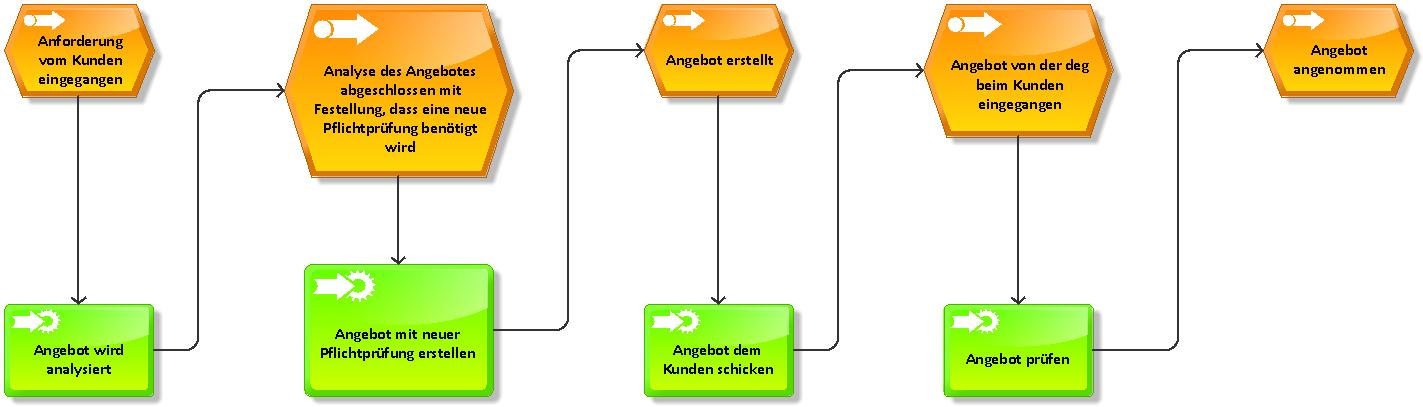
\includegraphics[scale=0.3]{anforderungundanalyse.jpeg}
\caption{Teilprozess:
Anforderung und Analyse}\label{Anforderung und Analyse}
\end{figure}



\subsection{Umsetzung}\label{TP2}
Nach der Annahme des Angebotes wird der Algorithmus f�r die neue Pflichtpr�fung
von einem Mitarbeiter der deg implementiert und die Pr�fungskonfiguration
definiert. Im Anschluss daran wird ein Codereview durch einem anderen
Mitarbeiter durchgef�hrt, um grobe Fehler bei der Implementierung
auszuschlie�en. Nachfolgend findet die Installation der Pflichtpr�fung statt, in
deren Anschluss entsprechende Tests durchgef�hrt werden. Nach erfolgreicher Testung ist dieser Teilprozess (Abbildung \ref{Umsetzung})
beendet.
\begin{figure}
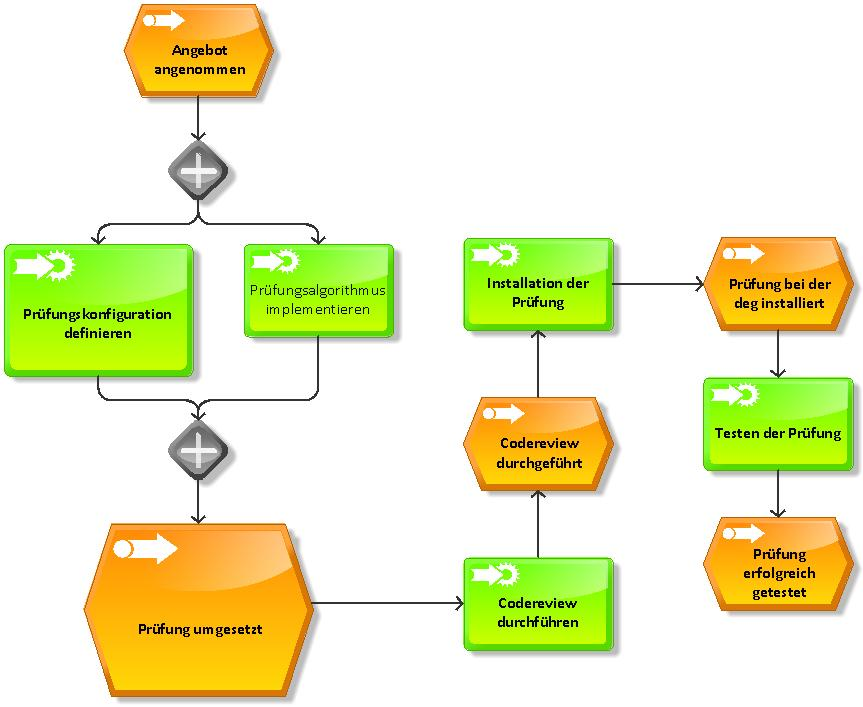
\includegraphics[scale=0.5]{umsetzung.jpeg}
\caption{Teilprozess:
Umsetzung}\label{Umsetzung}
\end{figure}



\subsection{Auslieferung}\label{TP3}
Der letzte Teilprozess wird haupts�chlich vom Kunden durchgef�hrt. Nach der
Auslieferung zum Kunden muss die Auslieferung dort installiert werden, bevor
mit dem Testen begonnen werden kann. Wird die Pr�fung positiv getestet, ist der
Prozess f�r die Betrachtung in diesem Praxisbericht beendet. Falls die Pr�fung
negativ getestet wurde, beginnt die Fehlersuche beim Kunden. Der Kunde kann
dabei nur einen Fehler bei der Installation der Pr�fung gemacht haben. Ist dies
der Fall, muss die Pr�fung neu installiert werden und der Test beginnt von
vorne. Falls der Fehler vom Kunden nicht nachvollziehbar ist, wird dieser Fehler
an die deg gemeldet. Dort beginnt eine neue Fehlersuche. Ausgehend davon, dass
wirklich eine Fehler vorliegt, gibt es hier zwei Fehlerursachen. Die erste
m�gliche Ursache bezieht sich auf die Implementierung des Pr�fungsalgorithmus
und die zweite m�gliche Ursache k�nnte eine falsche Definition der
Pr�fungskonfiguration sein. Je nachdem muss der konkrete Fehler gefunden,
behoben und neu an den Kunden ausgeliefert werden (Siehe Kapitel \ref{TP1} und
Kapitel \ref{TP2}). Dieser Prozess wird in Abbildung \ref{Auslierferung}
visualisiert.
\begin{figure}
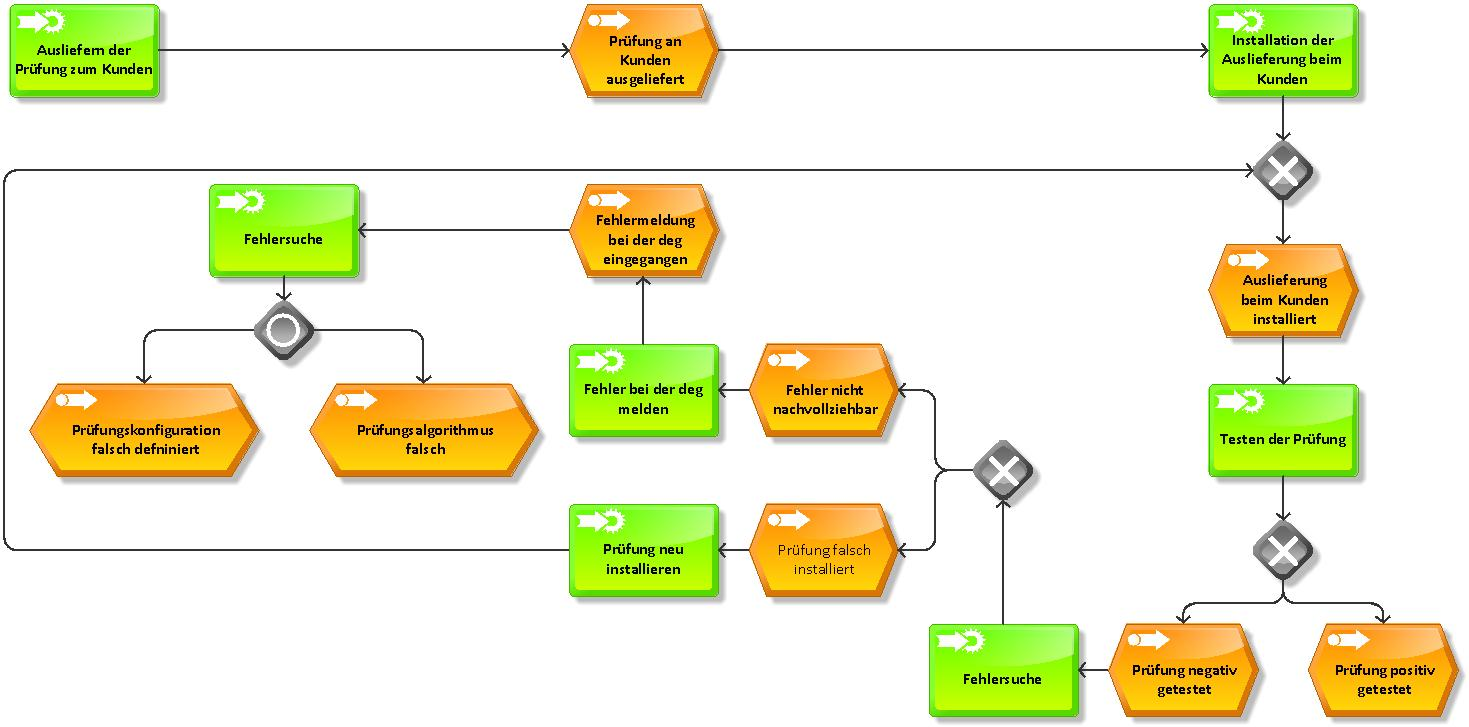
\includegraphics[scale=0.3]{auslieferung.jpeg}
\caption{Teilprozess:
Auslieferung}\label{Auslierferung}
\end{figure}



\subsection{Effizientere Workflows mit \emph{Xtext}}
Nach der Beschreibung des Gesamtprozesses wird nun betrachtet, welche Workflows
in diesem Prozess durch \emph{Xtext} effizienter gestaltet werden k�nnten. Im
ersten Teilprozess (siehe Kapitel \ref{TP1}) ist eine direkte
Effizientsteigerung\footnote{Direkt meint, dass sich eine �nderungen der
Workflows nicht direkt auf die Effizienz dieses Workflows auswirken w�rde.}
durch \emph{Xtext} nicht m�glich, da hier noch keine Implementierung vorgenommen
wird. Allerdings k�nnte eine gut lesbare Sprache, die f�r die Beschreibung der
Pflichtpr�fungen eingesetzt werden, die auch f�r der Beschreibung der Pr�fung im
Angebot zur Anwendung kommen kann. Somit k�nnte die Definition der
Pr�fungskonfiguration vom Angebot einfach �bernommen werden und m�sste nicht in
eine andere Syntax �bernommen werden. Insofern w�rde die Ver�nderung des
Workflows \emph{Angebot mit neuer Pflichtpr�fung erstellen} zu einer Zeit- und
Kosteneinsparung beim Workflow \emph{Pr�fungskonfiguration definieren} im
Teilprozess aus Kapitel \ref{TP2} f�hren.\\
Im zweiten Teilprozess (siehe Kapitel \ref{TP2}) kann \emph{Xtext} dabei helfen,
die Pr�fungskonfiguration zu definieren. Damit w�rde auch das Codereview f�r die
Definition der Pflichtpr�fungskonfiguration �berfl�ssig. Darauf wird sp�ter
nochmal eingegangen. Beim Testen der Pr�fung sehe ich keine M�glichkeit f�r die
Nutzung von \emph{Xtext}.\\
Im dritten Teilprozess (siehe Kapitel \ref{TP3}) w�re es durch den Einsatz von
\emph{Xtext} m�glich, die Fehlersuche zu vereinfachen. Nicht nur bei der deg k�nnten
Fehler in der Pr�fungskonfiguration schneller erkannt werden. Auch der Kunde
kann durch die Nutzung vo \emph{Xtext} seine Fehlersuche ausweiten. Im
sp�teren Verlauf wird auch darauf Bezug genommen.

\section{Analyse der Arbeitserleichterung}\label{Analyse der
Arbeitserleichterung}
Im vorherigen Kapitel wurden 4 Arbeitschritte ausfindig gemacht, die mittels
\emph{Xtext} direkt effizienter gestaltet werden k�nnen. 
\begin{enumerate}
\item Pr�fungskonfiguration definieren (siehe Kapitel \ref{TP2})
\item Codereview (siehe Kapitel \ref{TP2})
\item Fehlersuche (des Kunden, siehe Kapitel \ref{TP3})
\item Fehlersuche (der deg, siehe Kapitel \ref{TP3})
\end{enumerate}
\subsection{Effizienzsteigerung mit \emph{Xtext} durch eine Grammatik}
F�r die folgende Analyse wird in Betracht gezogen, dass f�r die Sprache zur
Definition von Prf�ngskonfigurationen eine Grammatik existiert, die von
\emph{Xtext} gelesen werden kann. Diese Grammatik wurde im Praxisbericht
\emph{Entwicklung einer Grammatik f�r eine DSL mit xText am Beispiel einer
Sprache zur Definition von Pflichtpr�fungen in profil c/s}\cite{pb5}
entwickelt. Um alle Konfigurationsdateien bzgl. der Syntax zu validieren, waren
noch einige Erweiterungen der Grammatik von N�ten (siehe Anhang
\ref{Grammatik}).
Beispielsweise mussten Kommentare in die Menge der Terminale aufgenommen werden.
\begin{lstlisting}[caption = Kommentare mit '\#' als Terminale]
terminal SL_COMMENT:
	'#' !('\n' | '\r')* ('\r'? '\n')?;
\end{lstlisting}
Dar�berhinaus wurden die Terminale zur Definition von \emph{Aktionen},
\emph{Wirkungen} und \emph{Klassennamen} auf die in profil c/s verwendeten
Bezeichnungen eingeschr�nkt. Listing \ref{wirkungen} zeigt dies f�r die
\emph{Wirkungen}. Die Umsetzung f�r die \emph{Aktionen} und \emph{Klassennamen}
ist analog dazu im Anhang \ref{Grammatik} zu finden.
\begin{lstlisting}[caption = Terminale f�r Wirkungen]
WIRKUNG:
	'VERHINDERT_AKTION' | 'OHNE' | 'WARNUNG';
\end{lstlisting}\label{wirkungen}
Erzeugt man mit \emph{Xtext} einen Editor, der die verwendete Syntax in den
Konfigurationsdateien hinsichtlich dieser Grammatik �berpr�ft, k�nnen dadurch
folgende Fehlerquellen ausgeschlossen werden.
\begin{itemize}
  \item Falscher struktureller Aufbau
  \item Zuweisung von Aktionen, die in profil c/s nicht existieren
  \item Zuweisung von Wirkungen, die in profil c/s nicht existieren
  \item Zuweisung von Klassennamen (Pr�fungsalgorithmen), die in profil c/s
  nicht existieren
\end{itemize}
Voraussetzung daf�r ist jedoch, dass \emph{Aktionen}, \emph{Wirkungen} und
\emph{Klassennamen} auch in der Grammatik gepflegt werden.\\
Die Arbeit w�re durch die wegfallenden Fehlerquellen effizienter. Dar�ber hinaus
muss der Entwickler auch nicht mehr nach dem vollqualifizierten Klassennamen
suchen, weil ihn dieser vom Editor vorgschlagen wird. Genauso verh�lt sich das
mit der Suche nach den richtigen Bezeichnungen f�r die \emph{Aktionen} oder
\emph{Wirkungen}\\
Beim Codereview muss dabei bedacht werden, dass damit noch keine semantik
validiert wird. Besnoders ist darauf zu achten, dass s�mtliche IDs korrekt
deklariert und zugewiesen sind.\\
Bei der Fehlersuche kann somit ein syntaktischer Fehler ausgeschlossen
werden.\footnote{Sollte es dennoch zu einem Syntaxfehler kommen, muss die
Grammatik angepasst werden.} Die Mitarbeiter der deg k�nnen sich bei der
Fehlersuche auf die fachliche Korrektheit der Pr�fungskonfiguration
konzentrieren. Der Kunde geniest bei der Fehlersuche dadurch derzeit kein
Vorteil. W�re der Kunde jedoch in der Lage die Konfigurationsdateien zu lesen
und zu verstehen, k�nnte auch dieser die Fachlichkeit der Pr�fungskonfiguration
pr�fen und sie mit dem Angebot abgleichen.\footnote{Neben einem Fehler in der 
Konfiguration kann auch ein vom Kunden nicht ausreichend gepr�ftes,
aber angenommenes Angebot zu einem nicht
erwarteten Ergebnis des Tests f�hren.}


\subsection{Effizienzsteigerung mit \emph{Xtext} durch Validierung}
Mittels Validierungen k�nnen bei \emph{Xtext} semantische Zusammenh�nge gepr�ft
werden. In dem Beispiel der Konfigurationsdateien werden alle Eigenschaften der
Pr�fungskonfigurationen �ber IDs zugewiesen. Die IDs, zu denen die Eigenschaften
zugewiesen werden, m�ssen in der Datei ein mal deklariert worden sein. Anderen
Falls ist die Zuweisung einer Eigenschaft �ber diese ID �berfl�ssig.\\
Ein weiterer semantischer Aspekt ist die Laufende Nummer, die bei der Zuweisung
mehrerer \emph{Wirkungen} und \emph{Aktionen} benutzt wird.\footnote{Genaueres
dazu ist im Praxisbericht \emph{Entwicklung einer Grammatik f�r eine DSL mit
xText am Beispiel einer Sprache zur  Definition von Pflichtpr�fungen in profil c/s}\cite{pb5} zu finden.}
\section{Fazit}
In diesem Bericht wurde gezeigt, dass durch den Einsatz von \emph{Xtext} einige
Fehlerquellen bei der Definition von Pr�fungskonfigurationen ausgeschlossen
werden k�nnen.
Voraussetzung daf�r ist jedoch eine gut definierte Grammatik, um eine  korrekte Syntax zuzusicher. Weiterhin bedarf
es f�r die Absicherung semantischer Zusammenh�nge entsprechende
Validierungsregeln. Mit \emph{Xtext} l�sst sich beides umsetzen und sehr
einfach in Eclipse intergrieren.\\
Durch den Ausschluss bestimmter Fehlerquellen l�sst sich bei den
Arbeitschritten, zu deren Unterst�tzung \emph{Xtext} eingesetzt werden kann
(genannt zu Beginn von Kaptiel \ref{Analyse der Arbeitserleichterung}), eine
Effizientsteigerung erzielen. Das hat auch eine Auswirkung auf den Gesamtprozess
(siehe Kapitel \ref{GP}). Auch das Durchf�hren von Prozessschleifen,
die Aufgrund von fehlgeschlagener Tests auftreten, wird im
Gesamtprozess reduziert.
Demnach wird der Prozess beim Einsatz von \emph{Xtext} schneller einen Endzustand erreichen.\\
Als zus�tzlichen Arbeitsaufwand k�nnte man die Pflege der Grammatik betrachten.
Diese muss immer aktualisiert werden, wenn \emph{Akionen} oder
\emph{Klassennamen} neu hinzukommen, oder wenn an den Bezeichnungen
der bestehenden \emph{Akionen} und
\emph{Klassennamen} etwas ge�ndert wird. Das Editieren der Grammatik ist jedoch
auch in Bezug auf diesen Aspekt ein Vorteil. Wenn die Grammatik ge�ndert wird,
werden in den Konfigurationsdateien an den entsprechenden Stellen Fehler
angezeigt. Dadurch entf�llt das Suchen entsprechender Stellen in den
Konfigurationsdateien, was bei vielen Konfigurationen ein erheblich gr��erer
Arbeitsaufwand w�re, als das �ndern einer Zeile in der Grammatik.

\pagenumbering{Roman}
\setcounter{page}{5}

\addcontentsline{toc}{section}{Literatur}
\bibliography{mybib}{}

\appendix
\section{Implementiertung}
\begin{lstlisting}[caption = Grammatik f�r die Syntax der Konfigurationsdateien]

\end{lstlisting}\label{Grammatik}
\end{document}
